\chapter{Метод оценки линейного искажающего оператора}
\section{Нахождение параметров искажения}
Как было сказано ранее, для восстановления изображения необходимо определить искажающий оператор. Он представляется дискретной импульсной характеристикой(ИХ). Однако такое представление не самое удачное, потому что это бесконечномерный вектор. Для эффективного поиска необходимо построить более удобную модель.

ИХ для вычислений представляется в виде матрицы. Простейшее представление смаза~--- линейный смаз\ref{eq:horizontalBlurPsf}.
\begin{equation}\label{eq:linearBlurArray}
\begin{pmatrix}
0 & 0 & 0 & 0.092 & 0.024\\
0 & 0.22 & 0.181 & 0.213 & 0.024\\
0.121 & 0.255 & 0.038 & 0 & 0\\
0.061 & 0 & 0 & 0 & 0
\end{pmatrix}
\end{equation}
Так например представляется в ИХ смаза длиной в 5 пикселей под углом $30^\circ$
\subsection{Кепстральный метод оценки линейного оператора}
Линейный смаз представляется величиной и углом смаза, альтернативное представление: координаты вектора смаза. 
Как уже было сказано ранее в разделе (\ref{seqtion:distortionModel}) по спектру искажённого изображения визуально можно определить величину и угол смаза.
\begin{figure}[h!]
	\begin{subfigure}[t]{0.3\textwidth}
		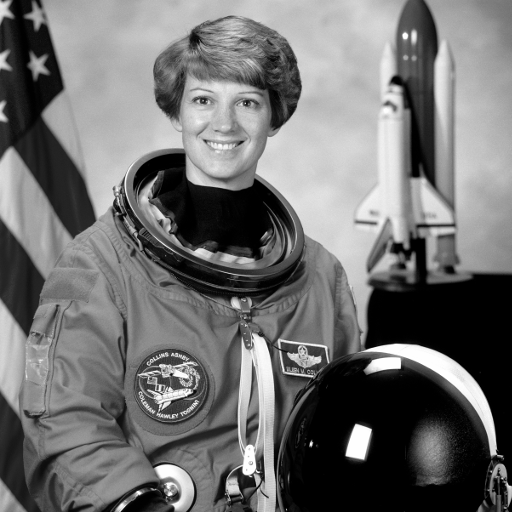
\includegraphics[width=\linewidth]{astro}
		\caption{исходное изображение}
	\end{subfigure}%
	\begin{subfigure}[t]{0.3\textwidth}
		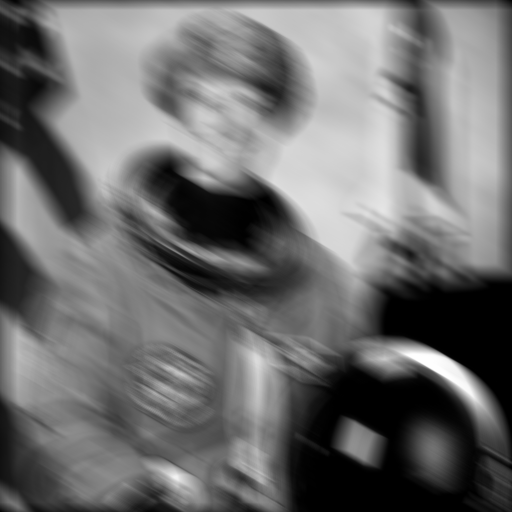
\includegraphics[width=\linewidth]{deconv-astro-blurred-shift40}
		\caption{смазанное изображение}
		\label{fig:astroShift40}
	\end{subfigure}%
	\begin{subfigure}[t]{0.3\textwidth}
		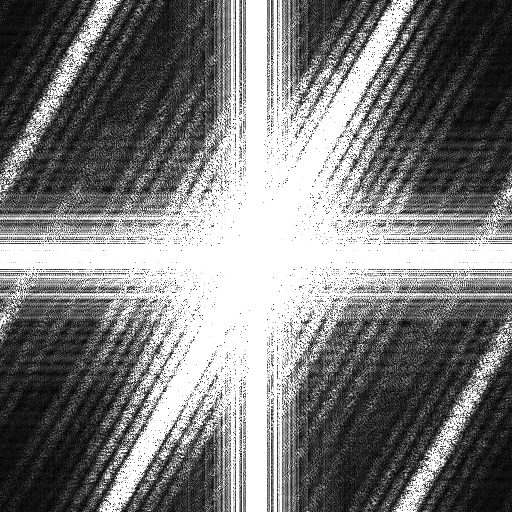
\includegraphics[width=\linewidth]{deconv-astro-spectre-shift40}
		\caption{спектр смазанного изображения}
		\label{fig:astroShift40Spectre}
	\end{subfigure}
	\caption{Смаз величиной в 40 пикселей под углом $330^{\circ}$}
	\label{fig:spectre}
\end{figure}
На рисунке \ref{fig:spectre} представлены оригинальное изображение, исходное изображение подвергнутое смазу и спектр смазанного изображения. По спектру \ref{fig:astroShift40Spectre} расстояние между чёрными полосами, в которых значение спектра близко к нулю является обратным к величине смаза. Также эти полосы ортогональны вектору смаза, угол наклона которого равен $30^\circ$. Однако, определение точных значений этих величин по частотному представлению изображения затруднительно. Для корректной работы методов восстановления изображения важно как можно точнее оценить ФРТ. Поэтому используют более точные способы определения параметров смаза.

Один из таких методов оценки параметров оператора линейного смаза основан на использовании кепстра изображения $\hat{f}(x,y)$~\cite{iterableImageRestorationBiemonLangdeik}
\begin{definition}\label{def:kepstr}
	\textbf{Кепстром $\hat{f}(x,y)$ изображения} называется обратное преобразование Фурье логарифма модуля преобразования Фурье.
	\begin{equation}
	\hat{g}(x,y) = F^{-1}\{log|F(u,v)|\},
	\end{equation}
\end{definition}
где $F^{-1}\{\cdot\}$~--- обратное преобразование Фурье, а $F(u,v)$~--- частотное представление изображения. Название <<кепстр>> получено перестановкой первых четырёх букв слова <<спектр>>.

Одним из основных свойств кепстра является то, что при свёртке двух сигналов их кепстры складываются. Таким образом, если
\begin{equation}
	g(x,y) = h(x,y) \conv f(x,y),
\end{equation}
то \cite{iterableImageRestorationBiemonLangdeik}
\begin{equation}\label{eq:kepstrSum}
	\hat{g}(x,y) = \hat{h}(x,y) + \hat{f}(x,y)
\end{equation}
При горизонтальном размытии ЧХ искажения можно записать в виде~\ref{eq:horizontalBlurIRFourier}:
\begin{equation*}
H(u,v) =       
\frac{1}{L+1}e^{-i\frac{L\pi}{N}m}\frac{\sin\frac{\pi(L+1)u}{N}}{\sin\frac{\pi u}{N}}
\end{equation*}
Она имеет нули в точках $\frac{N}{L+1}k, v$, где $k$~--- ненулевое целое, поэтому $\hat{h}(x,y)$ имеет большой отрицательный пик на расстоянии $L$ от начала координат. Следовательно у кепстра искажённого изображения он тоже будет, что сообщает о наличии искажения и его параметрах.
\begin{figure}[h!]
	\centerline{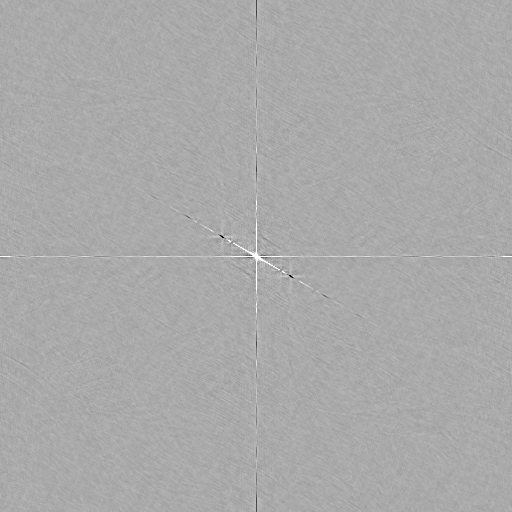
\includegraphics[width=0.5\linewidth]{deconv-kepstr-shift40-pi6}}
	\caption{Кепстр изображения смазанного на 40 пикселей под углом $330^{\circ}$.}
	\label{fig:kepstr}
\end{figure}

На рисунке \ref{fig:kepstr} изображён кепстр искажённого изображения \ref{fig:astroShift40}. В центре находится точка $(0,0)$. Симметрично относительно неё расположены отрицательные пики, характеризующие параметры смаза. Их координаты соответствуют вектору смаза.
Таким образом можно достаточно точно определить искажение. Отклонение от реальных значений достигает 1-2 пикселей.

\begin{figure}[h!]
	\centerline{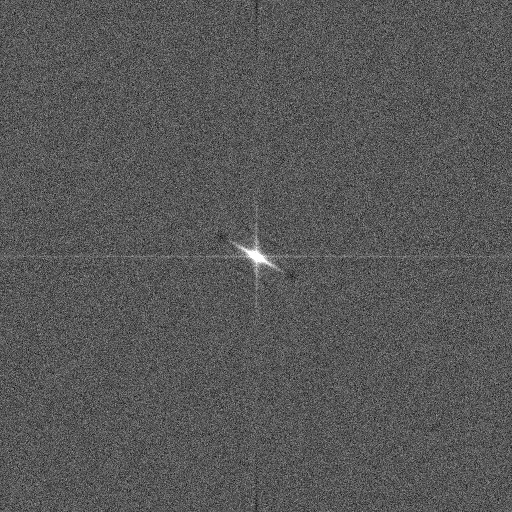
\includegraphics[width=0.5\linewidth]{deconv-kepstr-noised-shift40-pi6}}
	\caption{Кепстр изображения смазанного на 40 пикселей под углом $330^{\circ}$, зашумлённого с $\sigma=0,1$.}
	\label{fig:kepstrNoised}
\end{figure}
%%%% сослаться на диплом Кристины? Не это: ~\cite{panfilovaLinearBlur}
Кепстральный метод обладает рядом недостатков: в случае небольшого искажения (длина вектора размытия меньше 5 пикселей), точное определения смаза становится затруднительным. Также проблематично определить вектор смаза при большом шуме($\sigma_\eta \geq 5\cdot 10^{-2}$) Так как вклад шума слишком велик, минимум спектра приходится на случайную составляющую спектра, что видно на рисунке~\ref{fig:kepstrNoised}.

\subsection{Уточнение параметров искажения}
Кепстральный метод находит только целочисленные координаты вектора сдвига с погрешностью в несколько пикселей, тогда как на практике величина смаза есть число вещественное. Ниже будет рассмотрен алгоритм позволяющий уточнить параметры смаза.

Найти наилучшую оценку искажающего оператора~\ref{def:bestPsfEstimaton} невозможно, так как исходное изображение в общем случае неизвестно. Вместо этого можно минимизировать целевую функцию, а именно MSE конволюции оценки изображения и искажающего оператора относительно искажённого изображения. Тогда искомая ИХ $\hat{h}^*$ будет найдена по следующей формуле:
\begin{equation}\label{eq:bestPsf}
\hat{h}^* = \argmin_{\hat{h}} MSE(g, \phi(g,\hat{h}) \conv \hat{h}),
\end{equation}
где $\phi(g, h)$~--- результат применения деконволюции(используем метод Люси-Ричардсона) с оператором $h$.

Так как ИХ линейного смаза $h_{x_h,y_h}(x,y)$описывается координатами вектора смаза, минимизировать будем функцию двух переменных $x_h, y_h$.

\section{Нахождение параметров криволинейного искажающего оператора}
Криволинейный смаз будем представлять кривой Безье второго порядка
\subsection{Представление криволинейного искажающего оператора}
\subsection{Первое приближение}
\subsection{Второе приближение}
\subsection{Уточнение параметров}
\section{Выводы}
